\section{Experiment}

\subsection{Explanation of the experiment}
Once the equipment is ready, the experimental procedure can be carried out. The steps for conducting the measurements are as follows:

Measurement at room temperature: Begin by reading the resistivities of the samples at the initial temperature of 27.1. Record the obtained resistivity values.

Incremental Temperature Increase: Increase the temperature by 5 �C increments. Allow the system to stabilize at each new temperature setting before proceeding with measurements. At each temperature point, record the resistivities of the samples.

Temperature Range: Continue increasing the temperature until it reaches 100 �C, following the 5 �C increment pattern. Take note of the actual temperature of the samples, as it may vary slightly from the set value due to system variations.

\subsection{Uncertainties}

\large
\begin{itemize}
\item \begin{equation*}
	\Delta X = \frac{a}{100\%} \cdot X + n \cdot \Delta_{res}
\end{equation*}
\item \begin{equation*}
	u(t) = \frac{\Delta t}{\sqrt{3}}
\end{equation*}
\item \begin{equation*}
	u(t) = u(T)
\end{equation*}
\item \begin{equation*}
	u(1000/T) = 1000 \cdot \sqrt{\frac{u^2(T)}{T^4}}
\end{equation*}

\item \begin{equation*}
	u(ln(R)) = \frac{u(R)}{R}
\end{equation*}
\end{itemize}

For the metal objects, we need to plot the resistivity as a function of temperature in Kelvins and use linear regression method to find the coefficients a and b and their uncertainties u(a) and u(b):
\begin{equation*}
	R_m=f(t) =a \cdot t + b = R_0 \cdot \alpha \cdot t + R_0
\end{equation*}

$R_0, \alpha$ and their uncertainties are calculated as follows:


\begin{itemize}
	\item $R_0 = b$
	\item $u(R_0) = u(b)$
	\item $\alpha = frac{a}{R_0}$
	\item \begin{equation*}
		u(\alpha)= \sqrt{\frac{u^2(a)}{R_0^2} + \frac{a^2 \cdot 
		u^2(R_0)}{R_0^4} }
	\end{equation*}
\end{itemize}

For the semiconductor, we plot the natural logarithm of the resistivity as a function of 1000 over temperature in Kelvins and apply linear regression method to determine A, B, u(A) and u(B):

\begin{equation*}
	R_s=A \frac{1000}{T} + B = 10^-3 \cdot \frac{E_g}{2k} \cdot \frac{1000}{T} + ln(R_{s,0})
\end{equation*}

\subsection*{Data}

\subsubsection*{Initial data}

\begin{table}[!ht]
    \centering
    \begin{tabular}{c|c|c}
        $t[^\circ C]$ & $R_3[\Omega]$ & $R_4[\Omega]$ \\ \hline
        27.1 & 53.4 & 109.9 \\ 
        34.2 & 45.7 & 112.6 \\ 
        38 & 41.8 & 114.1 \\ 
        43.4 & 37 & 116.1 \\ 
        47.8 & 33.3 & 117.9 \\ 
        52.8 & 29.9 & 119.6 \\ 
        57.9 & 26.6 & 121.4 \\ 
        62.2 & 23.9 & 123.4 \\ 
        67 & 21.9 & 125.2 \\ 
        70.2 & 19.9 & 126.4 \\ 
        76.1 & 17.4 & 128.4 \\ 
        86.1 & 15.6 & 130.2 \\ 
        90.9 & 13.9 & 132.4 \\ 
        95.8 & 11.5 & 136.2 \\ 
        101 & 10.5 & 138.9 \\ 
    \end{tabular}
    \caption{Measurement data}
\end{table}

\subsubsection*{Semiconductor}

\begin{figure}[H]
	\centering
	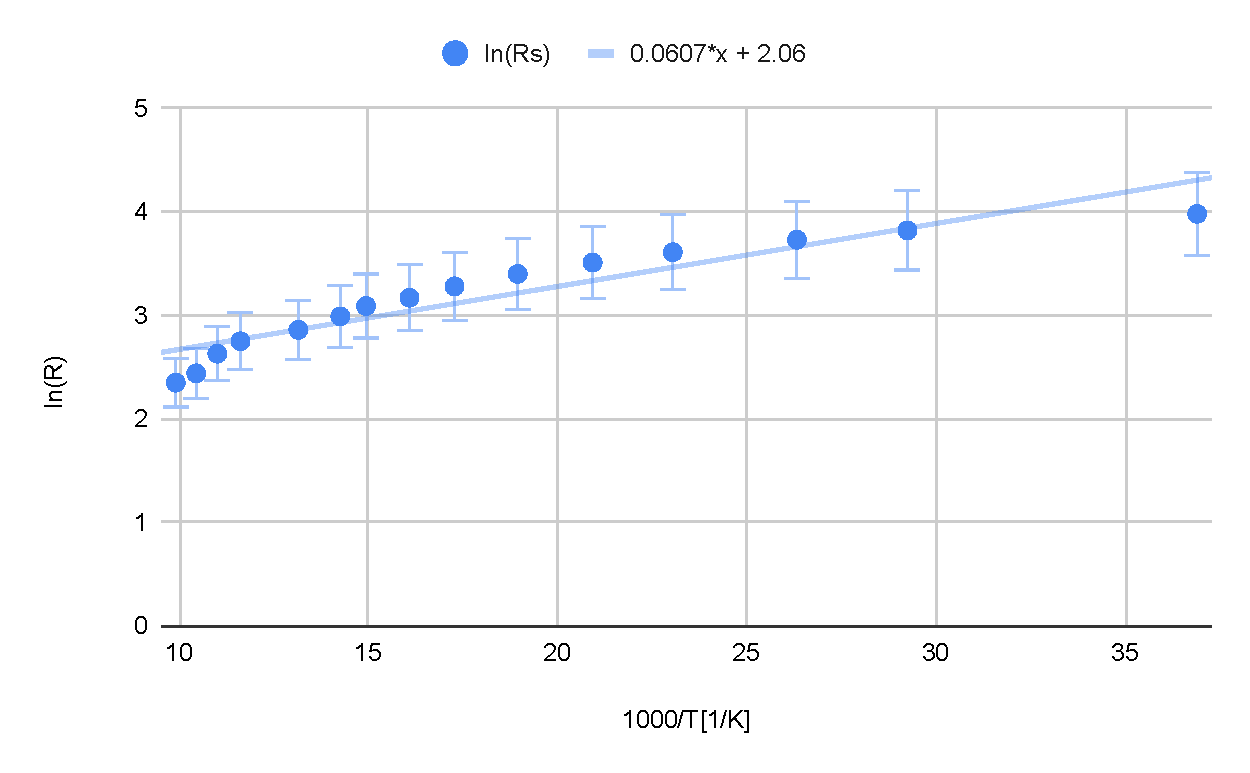
\includegraphics[width=12cm]{schematics/semi.pdf}
	
	
\end{figure}

\begin{table}[H]
    \centering
    \begin{tabular}{l|l|l}
        ~ & a & b \\ \hline
        ~ & 0.061 & 2.065 \\ 
        u(x) & 0.0063 & 0.125 \\ 
    \end{tabular}
    \caption{Linear regression }
\end{table}

\begin{table}[H]
    \centering
    \begin{tabular}{l|l|l|l|l}
        no. & t(C) & 1000/T[1/K] & R[$\Omega$] & ln(Rs) \\ \hline
        1 & 27.1 & 36.9 & 53.4 & 3.98 \\ 
        2 & 34.2 & 29.24 & 45.7 & 3.82 \\ 
        3 & 38 & 26.32 & 41.8 & 3.73 \\ 
        4 & 43.4 & 23.04 & 37 & 3.61 \\ 
        5 & 47.8 & 20.92 & 33.3 & 3.51 \\ 
        6 & 52.8 & 18.94 & 29.9 & 3.4 \\ 
        7 & 57.9 & 17.27 & 26.6 & 3.28 \\ 
        8 & 62.2 & 16.08 & 23.9 & 3.17 \\ 
        9 & 67 & 14.93 & 21.9 & 3.09 \\ 
        10 & 70.2 & 14.25 & 19.9 & 2.99 \\ 
        11 & 76.1 & 13.14 & 17.4 & 2.86 \\ 
        12 & 86.1 & 11.61 & 15.6 & 2.75 \\ 
        13 & 90.9 & 11 & 13.9 & 2.63 \\ 
        14 & 95.8 & 10.44 & 11.5 & 2.44 \\ 
        15 & 101 & 9.9 & 10.5 & 2.35 \\ 
        $\bar{X}$ & 63.37 & - & 26.82 & - \\ 
        $\Delta$X & 0.1 & - & 0.16 & - \\ 
        u(X) & 0.058 & - & 0.093 & ~ \\ 
        $u_c(X)$ & - & 0.025 & - & 0.0035 \\ 
    \end{tabular}
    \caption{Data Analysis}
\end{table}
\begin{table}[H]
    \centering
    \begin{tabular}{l|l|l|l}
        ~ & A[K] & Eg[J] & Eg[eV] \\ \hline
        ~ & 0.061 & 1.68E-21 & 2.065 \\ 
        u(X) & 0.0063 & - & - \\ 
        $u_c$(X) & ~ & 1.74E-22 & 0.125 \\ 
    \end{tabular}
    \caption{Data Analysis}
\end{table}

\subsubsection*{Metal}


\begin{figure}[H]
	\centering
	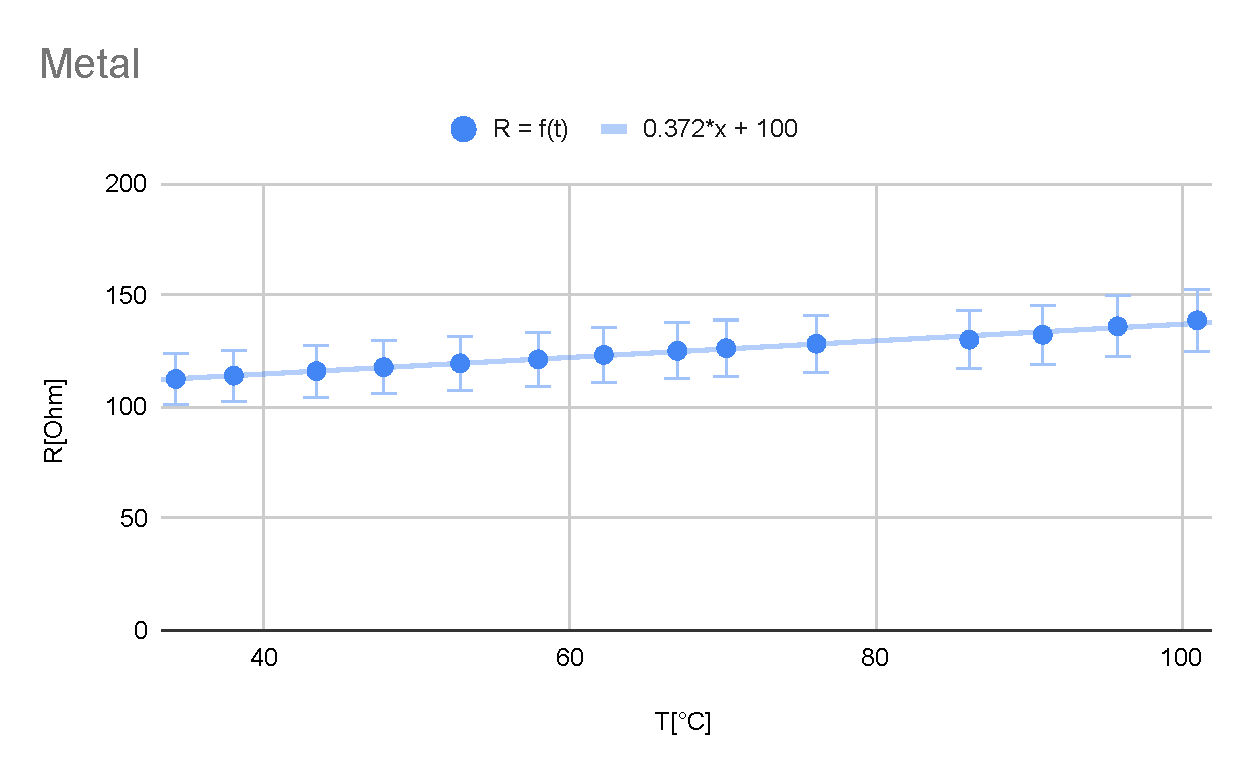
\includegraphics[width=12cm]{schematics/metal.pdf}
	
\end{figure}

\begin{table}[!ht]
    \centering
    \begin{tabular}{l|l|l}
        ~ & a & b \\ \hline
        ~ & 0.372 & 99.918 \\ 
        u(x) & 0.0089 & 0.595 \\ 
    \end{tabular}
    \caption{Linear regression}
\end{table}

\begin{table}[H]
    \centering
    \begin{tabular}{l|l|l|l|l|l}
        ~&T $[^\circ C^{-1}]$ & R[$\Omega$] & $a[\frac{\Omega}{^\circ C}$ & b, R0 & $\alpha [^\circ C^{-1}]$ \\ \hline
        1 & 27.1 & 109.9 & 0.372 & 99.918 & 0.003700 \\ 
        2 & 34.2 & 112.6 & ~ & ~ & ~ \\ 
        3 & 38 & 114.1 & ~ & ~ & ~ \\ 
        4 & 43.4 & 116.1 & ~ & ~ & ~ \\ 
        5 & 47.8 & 117.9 & ~ & ~ & ~ \\ 
        6 & 52.8 & 119.6 & ~ & ~ & ~ \\ 
        7 & 57.9 & 121.4 & ~ & ~ & ~ \\ 
        8 & 62.2 & 123.4 & ~ & ~ & ~ \\ 
        9 & 67 & 125.2 & ~ & ~ & ~ \\ 
        10 & 70.2 & 126.4 & ~ & ~ & ~ \\ 
        11 & 76.1 & 128.4 & ~ & ~ & ~ \\ 
        12 & 86.1 & 130.2 & ~ & ~ & ~ \\ 
        13 & 90.9 & 132.4 & ~ & ~ & ~ \\ 
        14 & 95.8 & 136.2 & ~ & ~ & ~ \\ 
        15 & 101 & 138.9 & ~ & ~ & ~ \\ 
        $\bar{X}$ & 63.37 & 123.51 & ~ & ~ & ~ \\ 
        $\Delta$X & 0.1 & 0.72 & - & - & - \\ 
        u (X) & 0.058 & 0.42 & 0.0089 & 0.595 & - \\ 
        $u_c$ (X) & - & - & - & - & 0.000092 \\ 
    \end{tabular}
    \caption{Data Analysis}
\end{table}


\subsection{Example Calculations}

\large
\begin{itemize}
\item \begin{equation*}
	\Delta X = \frac{0.5}{100\%} \cdot 10.5 + 1 \cdot 0.1 = 0.16 \Omega
\end{equation*}
\item \begin{equation*}
	u(t) = \frac{\Delta t}{\sqrt{3}} = \frac{0.1}{\sqrt{3}} = 0.058
\end{equation*}
\item \begin{equation*}
	u(t) = u(T) = 0.058
\end{equation*}
\item \begin{equation*}
	u(1000/T) = 1000 \cdot \sqrt{\frac{u^2(T)}{T^4}} = 1000 \cdot \sqrt{\frac{0.058^2}{63.37^4}} = 0.025
\end{equation*}

\item \begin{equation*}
	u(ln(R)) = \frac{u(R)}{R} = \frac{0.093}{26.82} =0.035 
\end{equation*}
\end{itemize}
